\documentclass[12pt]{article}

% Package
\usepackage{graphicx} % Add images package
\usepackage{listings} % Add code file package

% Document settings
\graphicspath{{../images}}
\setlength{\parindent}{0pt}

% Documentation title
\title{Sommatore a 3 input (v2)}
\author{Stefano Scarcelli \& Michele De Fusco}
\date{27 Dic 2023}


% Document
\begin{document}
% Cover
\maketitle
\newpage

% Indice
\tableofcontents
\newpage

% Document body

\section{Analisi progettuale}
    \subsection{Analisi preliminare}
        L'obbiettivo è quello di costruire un circuito in grado di sommare 3 numeri a \textit{n-bit} (\textit{2's complements}) e restituirne il risultato. Sia gli input che gli output devono essere sincronizzati tramite l'uso di registri.

        L'idea è quella di usare un sommatore 
        % #TODO: Nome tipo di sommatore.
    
    \subsection{Struttura del progetto}
        La struttura del progetto sarà fatta da un modulo che implementa i \textbf{registri} e un'altro dove viene implementato il circuito finale (\textbf{Three adder}).

\section{Implementazione}
    \subsection{Register n-bit}
        L'implementazione dell'\textbf{Register n-bit} è la medesima del progetto precedente (v1).

        \subsubsection{Codice VHDL}
           \lstinputlisting[language=vhdl, basicstyle=\footnotesize]{../../../Vivado_project_v1/Vivado_project_v1.srcs/sources_1/new/Register_n.vhd}
            
        \subsubsection{Sintesi}
            \begin{figure}[ht]
                \centering
                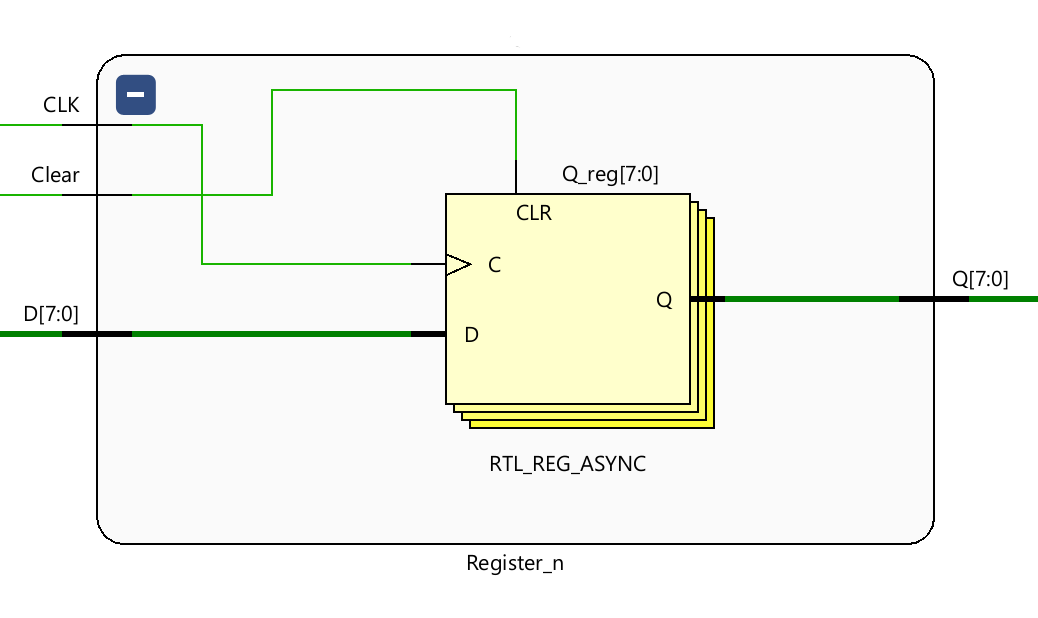
\includegraphics[scale=0.45]{Register.png}
                \caption{\textbf{Registro} a 8bit.}
            \end{figure}

    \subsection{Three adder (main)}
        % TODO

        \subsubsection{Codice VHDL}
            \lstinputlisting[language=vhdl, basicstyle=\footnotesize]{../../../Vivado_project_v1/Vivado_project_v1.srcs/sources_1/new/Three_Adder.vhd}
        
        \subsubsection{Sintesi}
            \begin{figure}[ht]
                \centering
                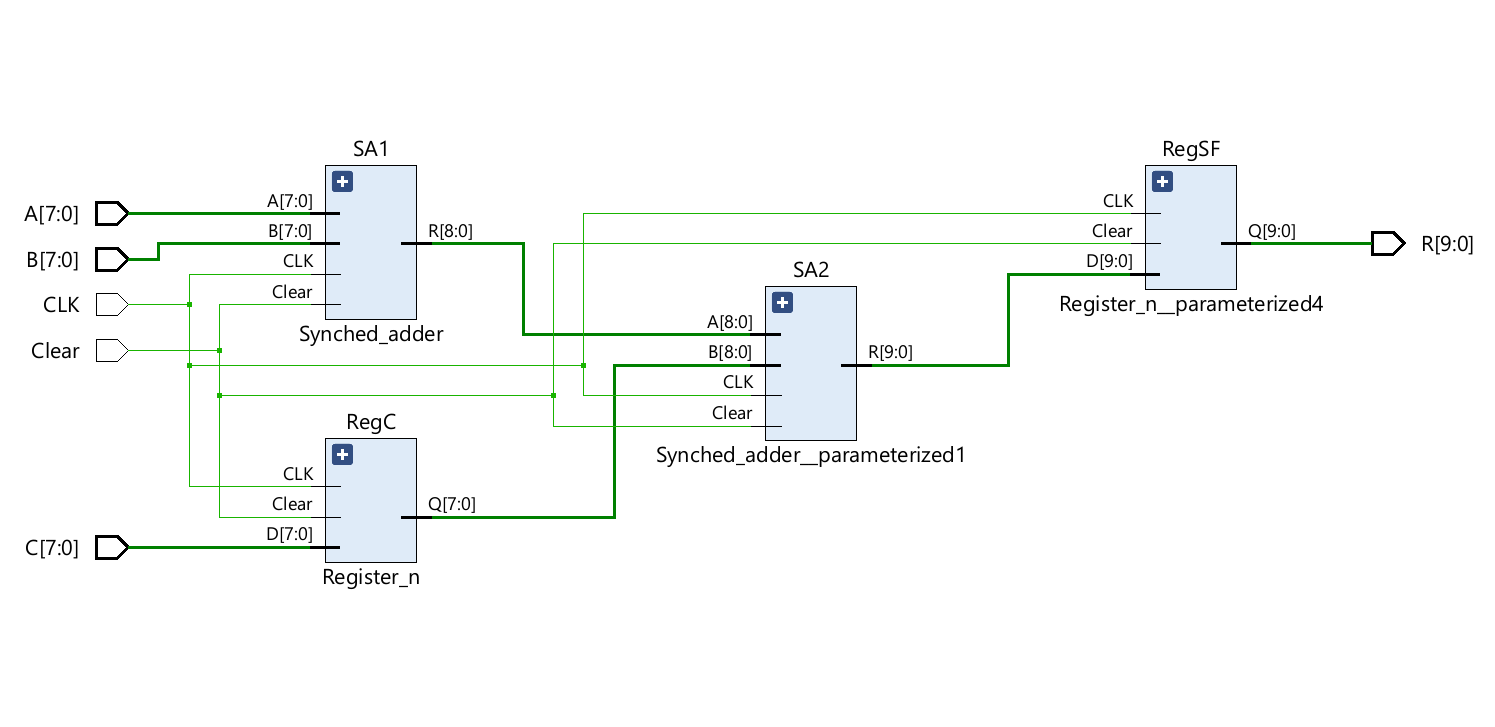
\includegraphics[scale=0.45]{main.png}
                \caption{Circuito principale.}
            \end{figure}

    \subsection{Time constraint}
        In più abbiamo aggiunto un \textit{time constraint} sul segnale di clock con un periodo di \textbf{5ns}.

        \begin{lstlisting}[basicstyle=\footnotesize]
            create_clock -period 5.000 -name main_clock
            -waveform {0.000 2.500} [get_nets CLK]
        \end{lstlisting}

        \subsubsection{Analisi del Time constraint}
            Con l'implementazione del codice abbiamo verificato (\textit{Timing summary routed}) che il \textbf{Time constraint} fosse valido, valutando di aver inserito un periodo di clock di superiore rispetto al minimo tollerabile dal circuito di \textbf{1.958ns}, rispetto dai \textbf{1.958ns} del progetto precedente (v1).

        \subsection{Risorse}
            \begin{figure}[ht]
                \centering
                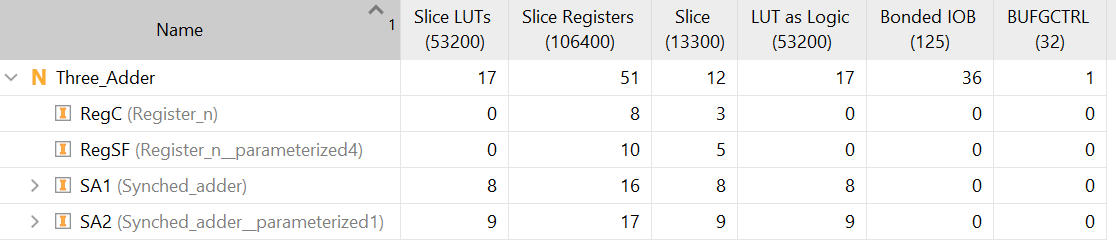
\includegraphics[scale=0.8]{Risorse_1.png}
                \caption{Risorse usate dai vari componenti.}
            \end{figure}

            \begin{figure}[ht]
                \centering
                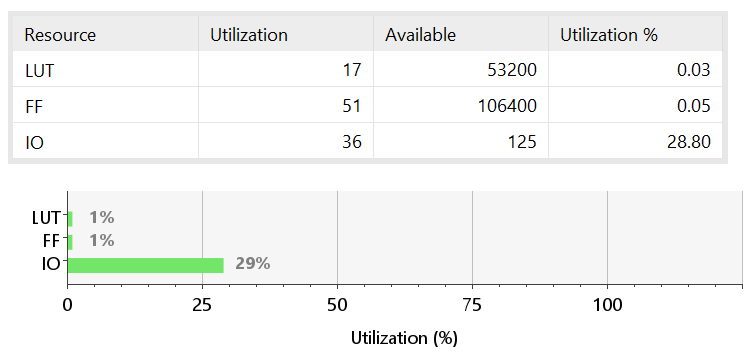
\includegraphics[scale=0.8]{Risorse_2.png}
                \caption{Riassunto delle risorse utilizzate.}
            \end{figure}

            \subsubsection{Potenza}
                \begin{figure}[ht]
                    \centering
                    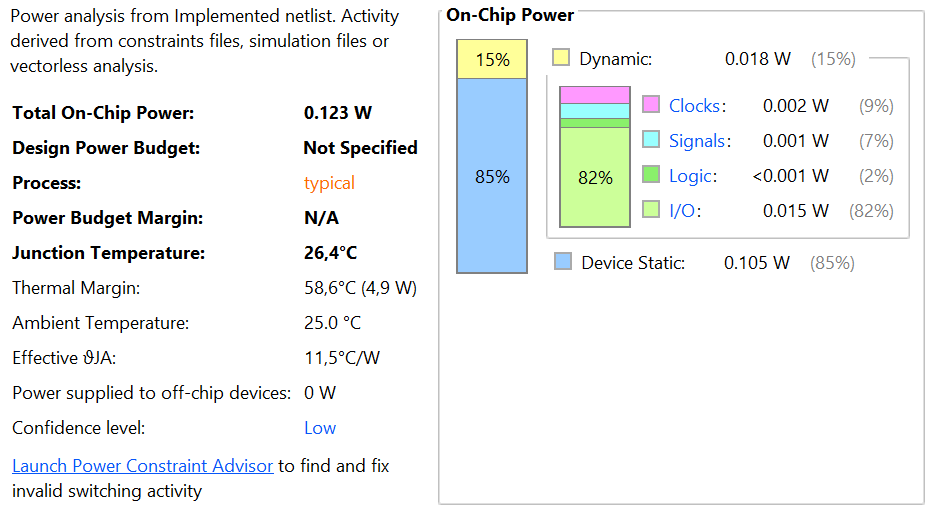
\includegraphics[scale=0.8]{Power.png}
                    \caption{Riassunto del report della potenza del circuito.}
                \end{figure}

\section{Testing}
    Per il test abbiamo deciso di usare il medesimo test del progetto precedente (v1).

    \subsection{Codice test test-bench}
        \lstinputlisting[language=VHDL, basicstyle=\footnotesize]{../../../Vivado_project_v1/Vivado_project_v1.srcs/sim_1/new/Sim_Add.vhd}

    \subsection{Risultati}
        I risultati delle simulazioni confermano il funzionamento del circuito come previsto.

        \subsubsection{Simulazione comportamentale}
            \begin{figure}[ht]
                \centering
                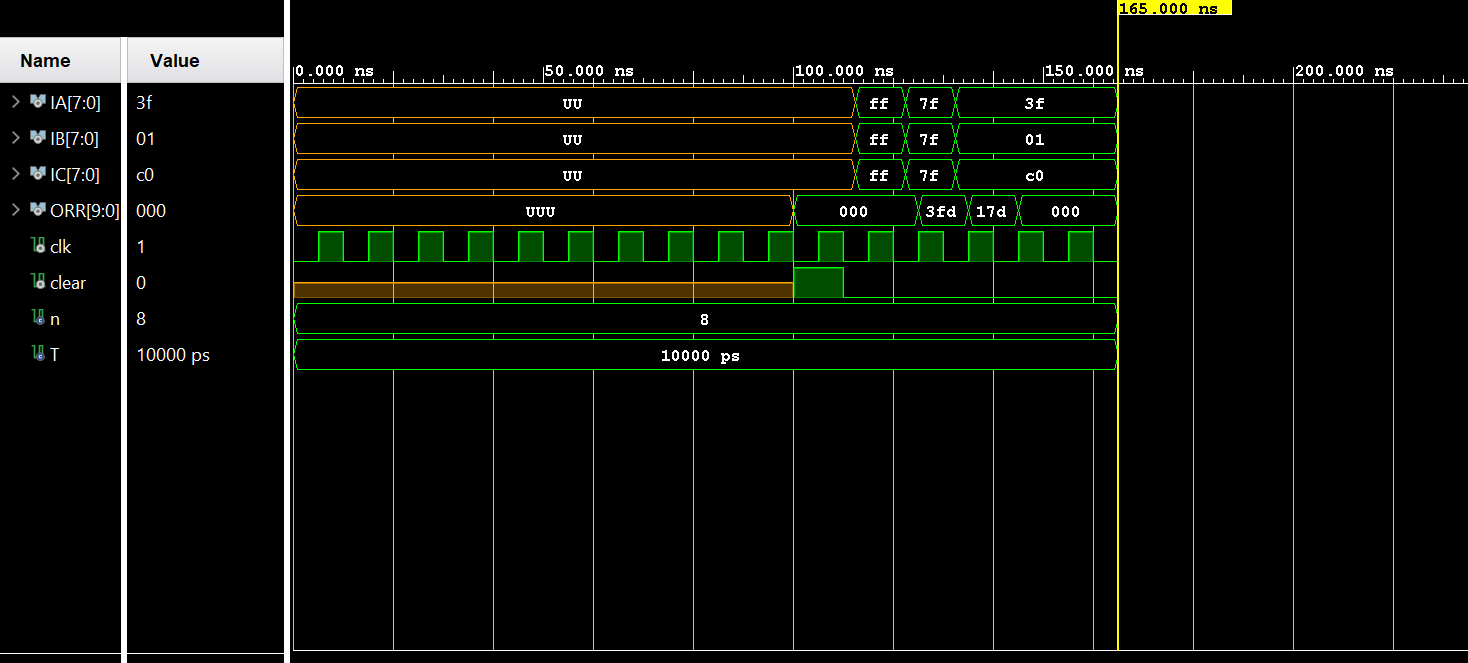
\includegraphics[scale=0.55]{Test_RTL.png}
                \caption{Grafico temporale simulazione comportamentale.}
            \end{figure}
            \newpage

        \subsubsection{Simulazione post sintesi}
            \begin{figure}[ht]
                \centering
                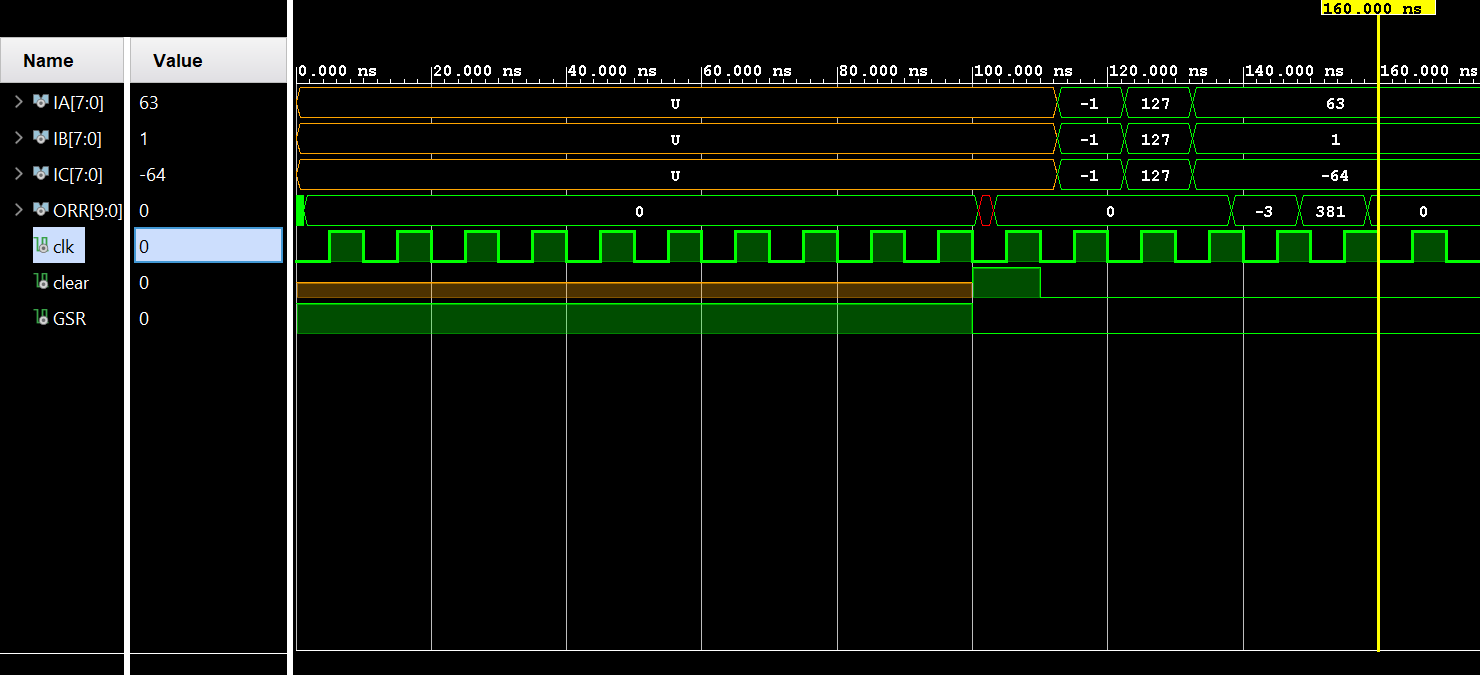
\includegraphics[scale=0.55]{Test_Sin.png}
                \caption{Grafico temporale simulazione post sintesi.}
            \end{figure}
            \newpage

        \subsubsection{Simulazione post implementazione}
            \begin{figure}[ht]
                \centering
                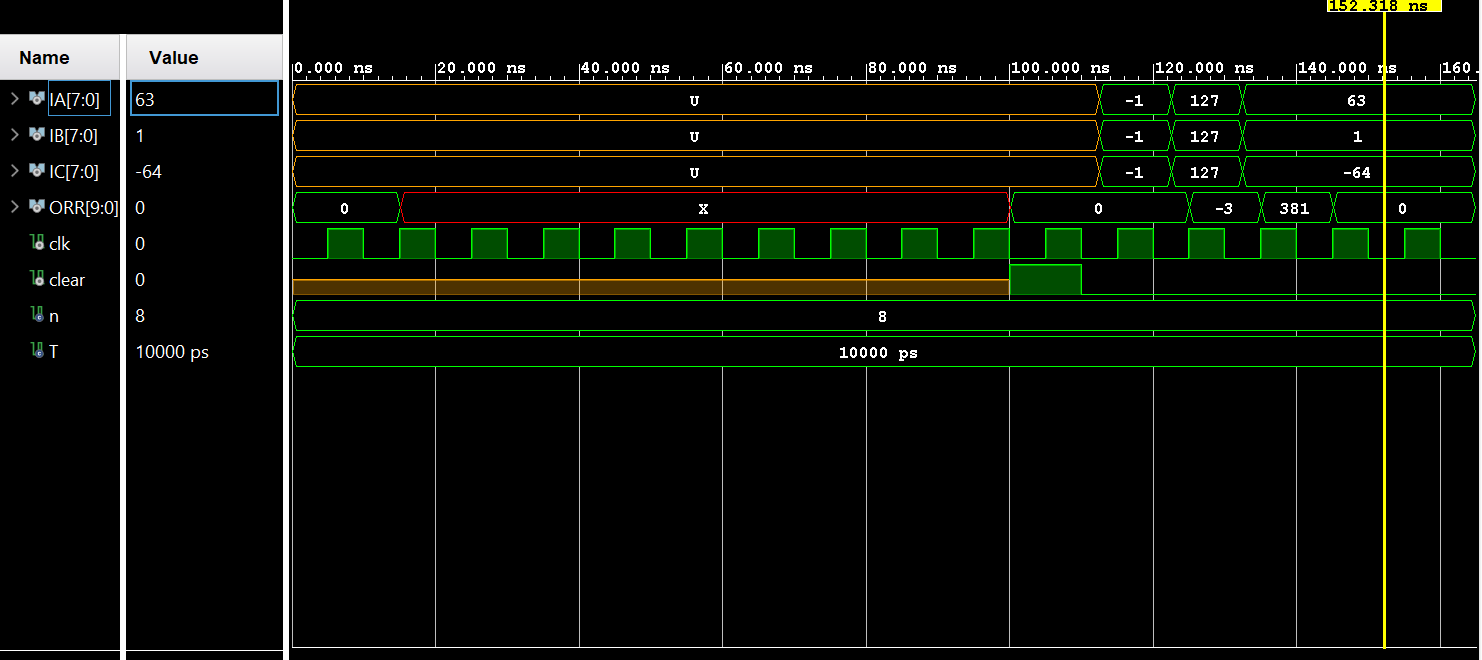
\includegraphics[scale=0.55]{Test.png}
                \caption{Grafico temporale simulazione post implementazione.}
            \end{figure}

\end{document}